\documentclass[12pt]{book}
\usepackage[utf8]{inputenc}
\usepackage[T1]{fontenc}
\usepackage{mathptmx}
\usepackage{geometry}
\usepackage{mathtools}
\usepackage[english]{babel}
\usepackage{graphicx}
\usepackage{subcaption}
\usepackage{stackengine}
\usepackage[os=win]{menukeys}
\usepackage{hyperref}
\usepackage{minted}
\usepackage{xcolor}
\usepackage{tikz}
\usepackage[yyyymmdd,hhmmss]{datetime}
\usepackage{etoolbox}
\usepackage[inline]{enumitem}
\usepackage{pdfpages}

\newcommand{\WindowsLogo}{\raisebox{-0.1em}{\includegraphics[height=0.8em]{images/logo/Windows_3_logo_simplified}}}
%\newcommand{\PowerLogo}{\raisebox{-0.1em}{\includegraphics[height=0.8em]{images/logo/power}}}
\newcommand{\WinKey}{\keys{\WindowsLogo}}
\newcommand{\PowerKey}{\keys{\PowerLogo}}

\patchcmd{\thebibliography}{\section*{\refname}}{}{}{}

\newcommand{\ShowOsVersion}{
	\immediate\write18{\unexpanded{foo=`uname -sro` && echo "${foo}" > tmp.tex}}
	\input{tmp}\immediate\write18{rm tmp.tex}
}

\newcommand{\ShowTexVersion}{
	\immediate\write18{\unexpanded{foo=`pdflatex -version | head -n1 | cut -d' ' -f1,2` && echo "${foo}" > tmp.tex}}
	\input{tmp}\immediate\write18{rm tmp.tex}
}

\addto\captionsenglish{\renewcommand{\contentsname}{Daftar Isi}}
\addto\captionsenglish{\renewcommand{\figurename}{Gambar}}

\hypersetup{
	colorlinks=true, %set true if you want colored links
	linktoc=all,     %set to all if you want both sections and subsections linked
	linkcolor=blue,  %choose some color if you want links to stand out
	urlcolor=blue,   %url color
}

\geometry{
	a4paper,
	left=10mm,
	right=10mm,
	top=15mm,
	bottom=15mm,
}

\title{\LARGE \bf
	Pengenalan MathWorks MATLAB dan Pemrogramannya\\
}

\author{}

\date{}

\hypersetup{citecolor=black}

\definecolor{LightGray}{gray}{0.95}

%\pagecolor[rgb]{0.1,0.1,0.1}
%\color[rgb]{1,1,1}

\begin{document}
	\frontmatter
	\maketitle
	
	%%%%%%%%%%%%%%%%%%%%%%%%%%%%%%%%%%%%%%%%%%%%%%%%%%%%%%%%%%%%%%%%%
	
	\newpage
	\tableofcontents
	
	%%%%%%%%%%%%%%%%%%%%%%%%%%%%%%%%%%%%%%%%%%%%%%%%%%%%%%%%%%%%%%%%%
	
	\newpage
	\chapter{Disclaimer}
	
	MATLAB adalah merek dagang dari The MathWorks, Inc.
	The MathWorks sendiri tidak menjamin akurasi isi buku ini.
	Penggunaan buku dalam kaitan perangkat lunak MATLAB tidak bermaksud promosi atau sponsor dari MathWorks.
	\\
	\\
	Konten buku ini disarikan dari buku \textit{"Chemical Engineering Computation with MATLAB"} oleh Yeong Koo Yeo,
	dipublikasikan oleh CRC Press tahun 2001.
	
	%%%%%%%%%%%%%%%%%%%%%%%%%%%%%%%%%%%%%%%%%%%%%%%%%%%%%%%%%%%%%%%%%
	
	\newpage
	\chapter{Penggunaan Buku}
	
	\section{Umum}
	Buku ini dibuat dengan tujuan penggunaan utama sebagai panduan digital.
	Anda tidak perlu mencetak buku ini ke bentuk kertas.
	Seluruh navigasi buku ini diharapkan menggunakan klik ke hyperlink di Daftar Isi,
	atau menggunakan tampilan \textbf{Index} yang tersedia di \textbf{SideBar} program pembaca PDF yang anda gunakan.
	
	\section{Petunjuk}
	Beberapa petunjuk yang digunakan di buku ini:
	\begin{itemize}
		\item \textbf{Cetak Tebal}: Menginformasikan identifier (keyword, variabel, fungsi, alamat, nama file, dst) yang berada di suatu paragraf
		\item \textit{Cetak Miring}: Bersama simbol panah (->) dan simbol lain, menginformasikan langkah-langkah klik menu/tombol.
		\item \textbf{TIPS:} Menginformasikan hal-hal yang dapat membantu atau pengetahuan tambahan.
		\item \textbf{PERINGATAN:} Menginformasikan hal-hal yang bener-benar harus diperhatikan.
	\end{itemize}

	\section{Penulisan Kode} 
	Untuk penulisan kode, akan digunakan tiga bentuk:
	\begin{itemize}
		\item IN dan OUT. Berupa bagian kode, dengan:
		\begin{itemize}
			\item Baris dengan tanda \textbf{Prompt} (>>) adalah Input
			\item Baris dibawahnya tanpa ada tanda \textbf{Prompt} (>>) adalah contoh Output
		\end{itemize}
	
		\begin{minted}[frame=lines,framesep=2mm,fontsize=\small,bgcolor=LightGray]{matlab}
>> input
output
		\end{minted}
	
		\item IN saja. Hanya sebagai input dengan ditandai \textbf{Prompt} (>>).
		Contoh Output disini tidak ditampilkan.
		
		\begin{minted}[frame=lines,framesep=2mm,fontsize=\small,bgcolor=LightGray]{matlab}
>> input
		\end{minted}
	
		\item Script/Function. Kode ditulis sebagai file script atau function tanpa ada tanda \textbf{Prompt} (>>) sama sekali.
		
		\begin{minted}[frame=lines,framesep=2mm,fontsize=\small,bgcolor=LightGray]{matlab}
function y=tambah(a,b)
	y = a + b
end
		\end{minted}
\end{itemize}
	
	%%%%%%%%%%%%%%%%%%%%%%%%%%%%%%%%%%%%%%%%%%%%%%%%%%%%%%%%%%%%%%%%%
	
	\newpage
	\mainmatter
	\chapter{Program MATLAB}
	
	Program MATLAB adalah program komputasi yang digunakan secara universal dalam bidang Sains dan Engineering.
	Secara garis besar, MATLAB adalah program kalkulator super canggih yang dapat menyelesaikan proses perhitungan kompleks.
	
	\section{Memulai Program}
	
	Anda dapat memulai program MATLAB sebagaimana program lainnya.
	
	\subsection{Windows}
	Untuk Windows 7, 8 , dan 10, Tekan tombol \textit{Start Windows} (\keys{\WindowsLogo}) dan ketik "MATLAB" untuk mencari program MATLAB yang terinstal.
	Tekan \textit{Enter} (\keys{\return}) untuk memulai
	\begin{figure}[!ht]
		\centering
		\includegraphics[width=250pt]{images/startmenuwin}
		\caption{Start MATLAB Windows}
	\end{figure}

	\subsection{GNU/Linux}
	Untuk GNU/Linux seperti ArchLinux, Manjaro, atau Ubuntu, tekan \textit{Start Menu} -> MATLAB.
	\begin{figure}[!ht]
		\centering
		\includegraphics[width=200pt]{images/startmenumate}
		\caption{Start MATLAB GNU/Linux}
	\end{figure}

	\newpage
	Metode lainnya adalah memanggil program matlab dengan Terminal/Bash Emulator dan masukkan perintah:
	\begin{minted}[frame=lines,framesep=2mm,fontsize=\small,bgcolor=LightGray]{bash}
$> matlab
	\end{minted}
	
	\subsection{MacOS}
	
	Menyusul
	
	\newpage
	\section{Bagian Antar Muka}
	
	Antar Muka (Interface) program MATLAB dapat berbeda antara satu pengguna dan pengguna lainnya.
	Berikut salah satu tampilan default yang umum dipakai:
	
	\begin{figure}[!ht]
		\centering
		\begin{subfigure}[b]{0.75\textwidth}
			\includegraphics[width=\textwidth]{images/matlabiface}
		\end{subfigure}
		\begin{subfigure}[b]{0.2\textwidth}
			\includegraphics[width=\textwidth]{images/matlabpart}
		\end{subfigure}
		\caption{Bagian Antar Muka}
	\end{figure}
	
	\subsection{Default Layout}
	
	Jika ingin untuk mengembalikan penataan (Layout) antar muka program, anda dapat melakukannya melalui Toolbar.
	Pilih tab \textit{Home} -> \textit{Layout}, kemudian pilih \textit{Default} atau \textit{Two-Column}.
	
	\begin{figure}[!ht]
		\centering
		\includegraphics[width=150pt]{images/matlablayout}
		\caption{Penataan MATLAB}
	\end{figure}
	
	\subsection{Toolbar}
	Toolbar disini bertindak sama seperti Toolbar pada Microsoft Office.
	Disini tersedia beragam perintah dalam bentuk icon yang dapat diklik.
	
	\newpage
	Tab yang tersedia antara lain:
	\begin{itemize}
		\item \textit{Home}. Berisi perintah dasar untuk mengolah file, variable, pengaturan program, dan layout.
		\item \textit{Plot}. Berisi perintah pengolahan plot langsung dari variable yang tersedia di Workspace.
		\item \textit{Apps}. Berisi perintah tambahan dari toolbox atau addon yang terinstal.
		\item \textit{Editor}. Berisi perintah untuk mengolah file, mengelola jalannya suatu skrip, dan perintah editing.
		Hanya muncul jika Editor diaktifkan.
		\item \textit{Publish}. Berisi perintah untuk membantu publikasi dan berbagi kode sumber melalui website MATLAB.
		Hanya muncul jika Editor diaktifkan.
		\item \textit{View}. Berisi perintah untuk mengolah tampilan kode sumber yang sedang diedit.
		Hanya muncul jika Editor diaktifkan.	
	\end{itemize}

	\subsection{Current Address}
	
	Current Address digunakan untuk menunjukkan alamat folder yang sedang aktif dan membantu navigasi berpindah folder.
	Icon tersedia antara lain panah navigasi (seperti pada webbrowser), icon folder untuk jelajah folder dengan program \textit{file-manager},
	teks alamat folder yang dapat diedit, icon panah bawah untuk history, dan icon lup untuk mencari.
	
	Untuk berpindah folder, anda dapat input teks alamat folder secara manual.
	Anda cukup klik alamat dan saat muncul cursor, anda dapat edit/paste alamat dan kemudian tekan Enter (\keys{\return}) untuk berpindah folder.
	
	\begin{figure}[!ht]
		\centering
		\includegraphics[width=300pt]{images/addressbaredit}
		\caption{Pindah Alamat}
	\end{figure}

	\textbf{TIPS:} Alamat di atas adalah format alamat untuk Unix (Linux/MacOS).
	Untuk Windows, alamant akan memiliki format dimulai C:$\backslash$ atau D:$\backslash$ sesuai drive.
	
	Selain itu, anda juga dapat menggunakan history untuk berpindah folder.
	Tekan icon panah bawah di sisi kanan alamat.
	
	\begin{figure}[!ht]
		\centering
		\includegraphics[width=300pt]{images/addressbarhistory}
		\caption{History Alamat}
	\end{figure}
	
	\newpage
	\subsection{Current Folder}
	
	Current Folder menampilkan file dan folder di alamat yang sedang aktif.
	Anda dapat membuka, menghapus, membuat, dan memindahkan file disini.
	Anda juga dapat berpindah folder dengan double-klik folder yang tersedia.
	
	\begin{figure}[!ht]
		\centering
		\includegraphics[width=150pt]{images/currentfolder}
		\caption{Current Folder}
	\end{figure}

	\subsection{Command Window}
	
	Command Window adalah bagian utama MATLAB dimana anda memasukkan perintah-perintah teks untuk diproses oleh MATLAB.
	Hasil proses juga akan ditampilkan disini.
	
	\begin{figure}[!ht]
		\centering
		\includegraphics[width=250pt]{images/commandwindow}
		\caption{Command Window}
	\end{figure}

	sebagai percobaan, coba masukkan perintah berikut dan tekan ENTER (\keys{\return})
	
	\begin{minted}[frame=lines,framesep=2mm,fontsize=\small,bgcolor=LightGray]{matlab}
>> a = 10^2
a = 
   100
	\end{minted}
	
	\subsubsection{Prompt}
	
	Prompt digunakan sebagai penanda baris dimana anda dapat memasukkan perintah ke MATLAB.
	Prompt memiliki dua mode:
	\begin{itemize}
		\item Ready. Berupa dua panah ke kanan (\textbf{>>}). Menandakan MATLAB siap menerima perintah.
		\item Busy.  Berupa dua panah ke bawah. Menandakan MATLAB sedang tidak siap menerima perintah.
	\end{itemize}

	\subsubsection{Suppress Output}
	
	\subsubsection{Menghentikan Proses}
	
	\subsubsection{History}
	
	\subsubsection{Sugesti}
	
	\subsection{Workspace}
	\subsection{Editor}
	
	
\end{document}